\documentclass[a4paper, 11pt, twoside]{article}
\usepackage{amssymb}
\usepackage{amsmath}
\usepackage{graphicx}
\begin{document}
\title{MATH6222 Week 8 Lecture Notes}
\author{Rui Qiu}
\date{2017-04-24}

\maketitle

\section{Monday}

Viewing times

Apr. 26 10:30-11:30, 3:00-4:00

Apr. 27 1-2

Apr. 28 10:30-11:30, 3:00-4:00\\

Midterm questions

Hand-deck probability $(5,4,3,1,)\rightarrow\frac{4{13\choose 5}3{13\choose 4}2{13\choose 3}13}{{52\choose 13}}$

But for $(5,4,4,0)\rightarrow\frac{4{13\choose 5}{3\choose 2}{13\choose 4}^2}{{52 \choose 13}}$

Bug-path problem

Suppose that $|a|+|b|\leq k, a, b$ have the same parity as $k$.

Then the bug can reach $(a,b)$ on day $k$.

Clearly, the bug can walk to $(a,b)$ in $|a|+|b|$ days. (By walking $a$ steps up/down if $a +/-$, and $b$ steps right/left if $b +/-$).

Note if $k$ has same parity as $a+b$, then it also has same parity as $|a|+|b|$.

Thus, $k-(|a|+|b|)$ is divisible by $2$.

If the bug walked up and down $\frac{k-(|a|+|b|)}{2}$ ?... then it lands on $(a,b)$ on day $k.$

...

If $(a,b)$ denotes the current position of the bug, then $|a|+|b|$ changes by at most $1$ each day. Thus on day $k$, $|a|+|b|\leq k$.

For parity, note that, the parity of $a+b$ changes every day, either from odd to even or from even to odd.

Thus the parity of $a+b$ is always the same as the parity of the day $k$.\\

\textbf{Problem:} Determine all integers satisfying $x^2\equiv 1\mod 5$.

$1,4,6,9,11,14,16,19,21,24,26,29\dots$

\begin{itemize}
	\item any integer where last digit is $1,4,6,9$
	\item all integers in congruence classes $1,4,6,9\mod 10$
	\item all integers in congruence classes $\overline{1}, \overline{4}\mod 5$
\end{itemize}

\textbf{Note:} If $x,y$ are in same congruence class $\mod 5$, then $x^2\equiv y^2\mod 5$.\\

Just need to figure out which congruence classes $\{\overline{0}, \overline{1}, \overline{2}, \overline{3}, \overline{4}\}\rightarrow\{\overline{0},\overline{1}, \overline{4}, \overline{4}, \overline{1}\}$

\[\mathbb{Z}_5\]

So solution is just all integers in these $2$ congruence classes $\overline{1}, \overline{4}\mod 5$\\

$2x=5\mod 5$ has no solutions in $\mathbb{Z}_6$.\\

\textbf{Key Question:} Given working $\mod n$, given congruence class $\overline{a}$. When can we find a $\overline{c}$ such that $\overline{c}\cdot\overline{a}=1$?

\section{Thursday}
\paragraph{Proposition:} Fix $n\in\mathbb{N}$. Suppose $a\in\mathbb{Z}$ satisfies $(a,n)=1$. Then $\exists\ b\in\mathbb{Z}$ such that $ab=1\mod n$.

Furthermore, $b$ is unique up to congruence $\mod n$. Equivalently, if $(a,n)=1$, then $\overline{a}\in\mathbb{Z}_n$ has a unique multiplicative inverse: $\exists\ ! \overline{b}\in\mathbb{Z}_n$ such that $\overline{a}\overline{b}=1$.

Notation: $(a,b)=\gcd(a,b)$.\\

\paragraph{Lemma:} Given $a,b,n\in\mathbb{Z}$, and suppose $(a,n)=1$. If $n|ab$, then $n|b$.

\paragraph{Proof:} $(a,n)=1$ means $a$ and $n$ have no prime factors in common. Therefore, the set of all prime factors of $n$ is contained in the set of all $1,\dots, ab$.

...\\

\paragraph{Proof of Proposition:} Consider multiples of $a \mod n$:

\[\{0\cdot a, 1\cdot a, 2\cdot a, \dots, (n-2)\cdot a\} = \{i\cdot a: 0\leq i\leq n-1\}\]

\paragraph{Claim:} These $n$ integers are all distinct $\mod n$.\\

$ia\equiv ja\mod n\iff n|(ia-ja)\iff n|a(i-j)\iff n|(i-j)$

(Use lemma in the last step)

This is impossible, because $i,j$ are distinct integers between $0$ and $n-1$. Therefore $i-j\not=0$ and $|i-j|\leq n-1$, so $i-j$ cannot be divisible by $n$.

This says we have a bijection from $\mathbb{Z}_n\rightarrow \mathbb{Z}_n$ by $\overline{x}\rightarrow \overline{a}\overline{x}.$\\

Since there are only $n$ congruence classes $\mod n$, every congruence class appears in this set

\[\{ia: 0\leq i \leq n-1\}\]

Therefore $\overline{1}$ is represented by some integers in this set:

We have $i\cdot a\equiv 1\mod n$ for some $0\leq i\leq n-1$.\\

\paragraph{Second Proof:}

By Euclidean algorithm,

 $\exists\ k, l\in\mathbb{Z}$ such that $ka+ln=1\iff ka\equiv 1\mod n$
 
 Suppose we are working with $\mod 17$, find $\overline{5}^{-1}$.
 
 $17=3\times 5+2, 5=2\times 2+1, 2=17-3\times 5.$
 
 $1=7\times 5-2\times 17$.
 
 $7\cdot 5\equiv 1\mod 17$
 
 $5x\equiv 3\mod 17$
 
 $x\equiv 7\cdot 5x\equiv 7\cdot 3\mod 17\equiv 4\mod 17.$\\
 
 \paragraph{Observation:} If $p$ is prime, then $1,\dots, p-1$ are all relatively prime to $p$.
 
\begin{itemize}
	\item This implies that \textbf{every} non-zero congruence class in $\mathbb{Z}_p$ has a multiplication inverse.
	\item $ax\equiv b\mod p$ ($a\not\equiv 0\mod p$) has a unique solution $\mod p$.
\end{itemize}

\paragraph{Fermat's Little Theorem:} Let $p$ be a prime. If $a\in\mathbb{Z}$ and $a\not\equiv 0\mod p$, then $a^{p-1}\equiv 1 \mod p$.

\paragraph{Proof:} Consider non-zero multiples of $a$: $1\cdot a, 2\cdot a, \dots, (p-1)\cdot a$. These are distinct and non-zero $\mod p$.

Multiply: $(1\cdot a)\cdot (2\cdot a)\cdots (p-1)\cdot a\equiv (p-1)!\mod p$

$\implies a^{p-1}\equiv 1 \mod p$.

Example (modulo 7): $5\cdot 10\cdot 15\cdots \cdot 30\equiv 6!\mod 7 $

\paragraph{Wilson's Theorem:} Let $p$ be a prime. Then $p|[(p-1)!+1]$.

Example: $p=5, [(p-1)!+1] = 25, 5|25.$

\paragraph{Proof:} In fact, $(p-1)!\equiv -1 \mod p$. (Try to prove this as a key step.)

$\overline{a}=1, 2, 3, 4, 5, 6$

$\overline{a}^{-1}=1, 4, 5, 2, 3, 6$

$6\cdot 5\cdot 4\cdot 3\cdot 2\cdot 1 \equiv 6\cdot 1\cdot 1\cdot 1 \equiv -1 \mod 7$

\paragraph{Lemma:} Fix $p$ prime, let $a\in\mathbb{Z}$ ($a\not\equiv 0\mod p$). Then $a^2\equiv 1 \mod p \iff a\equiv 1\mod p$ or $a\equiv -1 \mod p$.

\paragraph{Proof:} $a^2\equiv 1 \mod p\iff p|(a^2-1)\iff p|(a-1)(a+1) \iff p|(a-1)$ or $p|(a+1) \iff a\equiv 1 \mod p$ or  $a\equiv -1 \mod p$.

\paragraph{Proof of Wilson's Theorem:} Each of the integers $2,\dots, p-2$ pairs off with a unique inverse. Thus $2\cdot 3\cdots \cdot (p-2)\equiv 1\mod p$. Then $(p-1)!\equiv (p-1)\equiv -1\mod p$. We are done.

\section{Friday: Some miscellaneous}
\subsection{Permutations}
How many swaps do we need from 6-5-4-3-2-1 to 1-2-3-4-5-6?

3 swaps. 6 to 1, 5 to 2, then 4 to 3. How would you prove that you cannot do this in 2 swaps. If you have $2n$ numbers out of position, you at least need $n$ number of swaps to make then right. (Each swap changes at most 2 positions.)\\

How many swaps do we need from 2-3-4-5-6-1 to 1-2-3-4-5-6?

5 swaps.

2-3-4-5-1-6

2-3-4-1-5-6

2-3-1-4-5-6

2-1-3-4-5-6

1-2-3-4-5-6

But how to prove that 4 or 3 swaps cannot make this?

\paragraph{Definition:} A \textbf{permutation} of $[n]:\{1, 2, \dots, n\}$ is a bijection $f:[n]:[n]$.\\

The \textit{word form} of a permutation is the list $f(1), f(2), \dots, f(n)$.\\

A \textit{transposition} is just a permutation which swaps $i$ and $j$ (some $i, j \in [n]$) but leaves all other entries the same. Let $\sigma_{ij}:=$ transposition swapping integers $i,j$.\\

Let $f$ be the permutation associated to some out of order list. We seek a sequence of transpositions $\sigma_{i_1,j_1}, \sigma_{i_2,j_2}, \sigma_{i_3,j_3},\dots$ such that

\[\sigma_{i_k,j_k}\circ \sigma_{i_2, j_2} \circ\cdots\circ \sigma_{i_1, j_1}\circ f = \text{identity function}\]\\

$f(i)=j, f(j)=i, f(k)$, for all $k\not=i,j$.\\

Remark: Every transposition is its own inverse.\\

Therefore, $\iff f=\sigma_{i_1, j_1}\circ \sigma_{i_2,j_2}\circ\cdots\circ \sigma_{i_k,j_k}$.\\

Permutation is a map $f:[n]\rightarrow [n]$. So generally, given a function $f:A\rightarrow A$, we define the functional digraph of $f$ to be a graph with a vertex for every $a\in A$ and arrow from $f(a)\rightarrow f(a), \forall a\in A.$\\

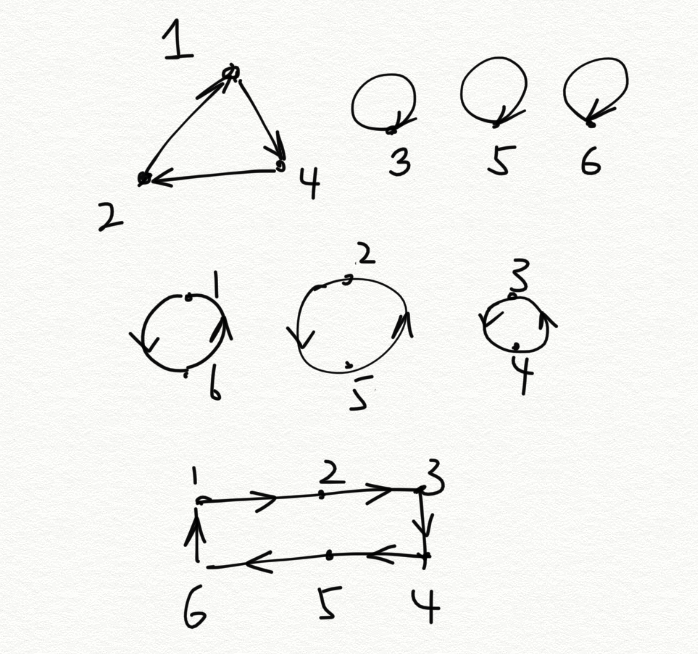
\includegraphics[width=\textwidth]{images/swaps}\\

Given a permutation $f$ whose digraph has $k$ cycles, the minimal number of swaps to sort it is $n-k$.\\

\paragraph{Proposition:} composing a permutation $f$ with a transposition $\sigma_{i,j}$, changes the digraph by adding $1$ cycle if $i,j$ are on the same cycle, deleting $1$ cycle if $i,j$ are on different cycles.\\

\subsection{Relation}

Let $S$ be a set. An \textbf{relation} on $S$ is a subset $R\subseteq S\times S$.

Example: 

$\{(x,y):x\leq y\}\subseteq R\times R$ ``$\leq$'' relation on $R$.

$\{(a,b):a|b\}\subseteq \mathbb{N}\times\mathbb{N}$ ``divisibility relation''.

Let $S$ be the set of all sets.

$\{(A, B): A\subseteq B\} \subseteq S\times S$

$\{(A, B): \exists\ \text{bijection}\ A \rightarrow B\}\subseteq S\times S$

Fix $n\in\mathbb{N}: \{(a, b): a\equiv b\mod n\}\subseteq \mathbb{Z}\times\mathbb{Z}$

Fix a permutation $f: \{(a, b): f^k(a)=b$ some $k\in\mathbb{N}\}\subseteq[n]\times [n]$\\

An \textbf{equivalence relation} is a relation which satisfies:

\begin{enumerate}
	\item $\forall x\in S, (x,x)\in R$. (reflexive)
	\item $\forall x, y\in S, (x,y)\in R\implies (y,x)\in R$. (symmetric)
	\item $\forall x, y, z \in S, (x,y)\in R \text{ and } (y,z)\in R \implies (x,z)\in R$. (transitivity)
\end{enumerate}

If $R$ is an equivalence relation, then for any $x\in S$, we can consider the ``equivalence class" of $x$. Notation:

\[\overline{X}=[x] = \{y\in S: y\sim x\}\]

Think about ``congruence class" in modulo arithmetic.

\end{document}